\subsection{CASE OF AN ORDERED GROUP OF DEGREES}

An order structure (denoted by \(\leqslant\) ) on a commutative group \(\Delta\) written additively is said to be compatible with the group structure if, for all \(\rho\in\Delta\) , the relation \(\lambda\leqslant\mu\) implies \(\lambda+\rho\leqslant\mu+\rho\) . The group \(\Delta\) with this order structure is then called an ordered group. We shall study these groups in detail in VI, §1; here we restrict ourselves to the remark that in such a group the relation \(\lambda>0\) implies \(\lambda+\mu>\mu\) for all \(\mu\) , for it implies \(\lambda+\mu\geqslant\mu\) by definition and the relation \(\xi+\mu=\mu\) is equivalent to \(\xi=0\) .

Let \(\Delta\) be an ordered commutative group, A a graded ring of type \(\Delta\) and \((\mathbf{A}_{\lambda})\) its graduation and suppose that the relation \(\mathbf{A}_{\lambda} \neq \{0\}\) implies \(\lambda \geqslant 0\) ; then it follows from the definitions that \(\mathfrak{I}_0 = \sum_{\lambda > 0} \mathbf{A}_{\lambda}\) is a graded two-sided ideal of A, by virtue of the remark made above.

PROPOSITION 6. Let \(\Delta\) be an ordered commutative group, A a graded ring of type \(\Delta\) , \((\mathbf{A}_{\lambda})\) its graduation, M a graded A-module of type \(\Delta\) and \((\mathbf{M}_{\lambda})\) its graduation. Suppose that the relation \(\mathbf{A}_{\lambda} \neq \{0\}\) implies \(\lambda \geqslant 0\) and that there exists \(\lambda_0\) such that \(\mathbf{M}_{\lambda_0} \neq \{0\}\) and \(\mathbf{M}_{\lambda} = \{0\}\) for \(\lambda < \lambda_0\) . Then, if \(\Im_0 = \sum_{\lambda > 0} \mathbf{A}_{\lambda}\) , \(\Im_0 \mathbf{M} \neq \mathbf{M}\) .

Let \(x\) be a non-zero element of \(\mathbf{M}_{\lambda_0}\) ; suppose that \(x \in \mathfrak{I}_0\mathbf{M}\) . Then \(x = \sum_{i} a_i x_i\) , where the \(a_i\) are homogeneous elements \(\neq 0\) of \(\mathfrak{I}_0\) and the \(x_i\) homogeneous elements \(\neq 0\) of \(\mathbf{M}\) with \(\deg(x) = \deg(a_i) + \deg(x_i)\) for all \(i\) (no. 2). But, as \(\deg(a_i) > 0\) , \(\lambda_0 = \deg(a_i) + \deg(x_i) > \deg(x_i)\) , which contradicts the hypothesis.

COROLLARY 1. With the hypotheses on \(\Delta\) and A of Proposition 6, if \(M\) is a finitely generated graded A-module such that \(\mathfrak{S}_0\mathbf{M} = \mathbf{M}\) , then \(\mathbf{M} = \{0\}\) .

Suppose \(M \neq \{0\}\) . Let \(\lambda_{0}\) be a minimal element of the set of degrees of a finite generating system of M consisting of homogeneous elements \(\neq0\) ; then the hypotheses of Proposition 6 would be fulfilled, which implies a contradiction.

COROLLARY 2. With the hypotheses on \(\Delta\) and A of Proposition 6, let M be a finitely generated graded A-module and N a graded submodule of M such that \(N + I_{0}M = M\) ; then N = M.

M/N is a finitely generated graded A-module and the hypothesis implies that \(\mathfrak{S}_{0}(\mathbf{M}/\mathbf{N}) = \mathbf{M}/\mathbf{N}\) ; hence M/N = 0.

COROLLARY 3. With the hypotheses on \(\Delta\) and A of Proposition 6, let \(u: \mathbf{M} \to \mathbf{N}\) be a graded homomorphism of graded right A-modules, where N is assumed to be finitely generated. If the homomorphism

\[
u \otimes 1: \mathbf {M} \otimes_ {\mathbf {A}} (\mathbf {A} / \mathfrak {I} _ {0}) \rightarrow \mathbf {N} \otimes_ {\mathbf {A}} (\mathbf {A} / \mathfrak {I} _ {0})
\]

is surjective, then u is surjective.

\(u(\mathbf{M})\) is a graded submodule of \(\mathbf{N}\) and the \((\mathbf{A} / \mathfrak{I}_0)\) -module

\[
(\mathbf {N} / u (\mathbf {M})) \otimes_ {\mathbf {A}} (\mathbf {A} / \mathfrak {I} _ {0})
\]

is isomorphic to \((\mathbf{N} \otimes_{\mathbf{A}} (\mathbf{A} / \mathfrak{I}_0)) / \mathrm{Im}(u \otimes 1)\) (§ 3, no. 6, Proposition 6). The hypothesis therefore implies \((\mathbf{N} / u(\mathbf{M})) \otimes_{\mathbf{A}} (\mathbf{A} / \mathfrak{I}_0) = 0\) and hence \(\mathbf{N} = u(\mathbf{M})\) by Corollary 1.

Remark. It follows from the proof of Corollary 1 that Corollaries 1 and 2 (resp. Corollary 3) are still valid when, instead of assuming that M (resp. N) is finitely generated, the following hypothesis is made: there exists a subset \(\Delta^{+}\) of \(\Delta\) satisfying the following conditions:

\begin{enumerate}
\def\labelenumi{(\arabic{enumi})}
\item
  for \(\lambda \notin \Delta^{+}\) , \(\mathbf{M}_{\lambda} = \{0\}\) (resp. \(\mathbf{N}_{\lambda} = \{0\}\) );
\item
  every non-empty subset of \(\Delta^{+}\) has a least element.
\end{enumerate}

This will be the case if \(\Delta = Z\) and M (resp. N) is a graded module with positive degrees.

PROPOSITION 7. Suppose that \(\Delta = \mathbf{Z}\) . With the hypotheses on A and M of Proposition 6, consider the graded \(\mathbf{A}_0\) -module \(\mathbf{N} = \mathbf{M} / \Im_0\mathbf{M}\) and suppose the following conditions hold:

\begin{enumerate}
\def\labelenumi{(\roman{enumi})}
\item
  each of the \(\mathbf{N}_{\lambda}\) considered as an \(\mathbf{A}_0\) -module admits a basis \((y_{\iota \lambda})_{\iota \in I_{\lambda}}\) ;
\item
  the canonical homomorphism \(\mathfrak{S}_0\otimes_{\mathbf{A}}\mathbf{M}\to \mathbf{M}\) is injective.
\end{enumerate}

Then \(\mathbf{M}\) is a graded free A-module (no. 2, Remark 3) and, to be precise, if \(x_{\iota \lambda}\) is an element of \(\mathbf{M}_{\lambda}\) whose image in \(\mathbf{N}_{\lambda}\) is \(y_{\iota \lambda}\) , the family \((x_{\iota \lambda})_{(\iota ,\lambda)\in \mathbf{I}}\) (where \(\mathbf{I}\) is the set the sum of the \(\mathbf{I}_{\lambda}\) ) is a basis of \(\mathbf{M}\) .

We know (no. 2, Remark 3) that there is a graded free A-module L (of graduation \((\mathbf{L}_{\lambda})\) ) and a surjective homomorphism \(p: \mathbf{L} \to \mathbf{M}\) of degree 0 such that \(p(e_{t\lambda}) = x_{t\lambda}\) for all \((t, \lambda) \in \mathbf{I} ((e_{t\lambda})_{(t,\lambda) \in \mathbf{I}}\) being a basis of L consisting of homogeneous elements \(e_{t\lambda} \in \mathbf{L}_{\lambda}\) . It follows from the above Remark that \(p\) is surjective. Consider the graded A-module \(\mathbf{R} = \operatorname{Ker}(p)\) and note that \(\mathbf{R}_{\lambda} = \{0\}\) for \(\lambda < \lambda_0\) by definition; we need to prove that \(\mathbf{R} = \{0\}\) and by Proposition 6 it will suffice to show that \(\mathfrak{S}_0\mathbf{R} = \mathbf{R}\) . Consider the commutative diagram (§ 3, no. 6, Proposition 5)

\pandocbounded{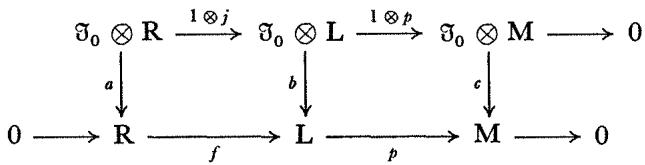
\includegraphics[keepaspectratio]{images/part003_24c814e1.jpg}}

where \(j\) is the canonical injection, \(a, b, c\) deriving from the canonical injection \(\mathfrak{I}_0 \to \mathbf{A}\) ( \(\S 3\) , no. 4, Proposition 4); it must be shown that \(a\) is surjective. Note that, as \(\mathbf{L}\) is free, \(b\) is injective ( \(\S 3\) , no. 7, Corollary 6 to Proposition 7) and \(c\) is injective by hypothesis. Then let \(t\) be an element of \(\mathbf{R}\) and \(t\) its class in \(\mathbf{R} / \mathfrak{I}_0\mathbf{R}\) ; then there is an exact sequence ( \(\S 3\) , no. 6, Proposition 5 and Corollary 2 to Proposition 6)

\[
\mathrm{R} / \mathfrak {I} _ {0} \mathrm{R} \xrightarrow {\jmath} \mathrm{L} / \mathfrak {I} _ {0} \mathrm{L} \xrightarrow {\bar {p}} \mathrm{M} / \mathfrak {I} _ {0} \mathrm{M} \longrightarrow 0
\]

where \(j\) and \(\bar{p}\) derive from \(j\) and \(p\) when passing to the quotients and \(\bar{p}\) is by hypothesis a bijection; then \(\bar{j}(t) = 0\) , in other words \(j(t) \in \mathfrak{I}_0\mathbf{L}\) . Then there is an element \(z \in \mathfrak{I}_0 \otimes \mathbf{L}\) such that \(j(t) = b(z)\) ; as \(p(b(z)) = 0\) , \(c((1 \otimes p)(z)) = 0\) and, as \(c\) is injective, \((1 \otimes p)(z) = 0\) . In other words, \(z\) is the image of an element \(t' \in \mathfrak{I}_0 \otimes \mathbf{R}\) under \(1 \otimes j\) and then \(j(a(t')) = b(z) = j(t)\) ; as \(j\) is injective, this implies \(t = a(t')\) .

We shall show later (Commutative Algebra, II, § 3, no. 2, Proposition 5) how this proposition can be extended to non-graded modules.

Lemma 1. For a commutative group \(\Delta\) to be such that there exists on \(\Delta\) a total ordering compatible with the group structure of \(\Delta\) , it is necessary and sufficient that \(\Delta\) be torsion-free.

If there exists such an order structure on \(\Delta\) and if \(\lambda > 0\) , then \(\lambda + \mu > 0\) for all \(\mu \geqslant 0\) and in particular, by induction on the integer \(n > 0\) , \(n.\lambda > 0\) , which proves that \(\Delta\) is torsion-free (since every element \(\neq 0\) of \(\Delta\) is either \(>0\) or \(< 0\) ). Conversely, if \(\Delta\) is torsion-free, \(\Delta\) is a sub- \(\mathbf{Z}\) -module of a vector \(\mathbf{Q}\) -space ( \(\S 7\) , no. 10, Corollary 1 to Proposition 26) which may be assumed of the form \(\mathbf{Q}^{(I)}\) ; if I is given a well-ordering (Set Theory, III, \(\S 2\) , no. 3, Theorem 1) and \(\mathbf{Q}\) its usual ordering, the set \(\mathbf{Q}^{(I)}\) with the lexicographical ordering is totally ordered (Set Theory, III, \(\S 2\) , no. 6); it is immediate that this ordering is compatible with the additive group structure of \(\mathbf{Q}^{(I)}\) .

PROPOSITION 8. Let \(\Delta\) be a torsion-free commutative group and A a graded ring of type \(\Delta\) . If the product in A of two homogeneous elements \(\neq 0\) is \(\neq 0\) , the ring A has no divisor of 0.

Let \(\Delta\) be given a total ordering compatible with its group structure (Lemma

\begin{enumerate}
\def\labelenumi{\arabic{enumi})}
\tightlist
\item
  and let \(x = \sum_{\lambda \in \Delta} x_{\lambda}, y = \sum_{\lambda \in \Delta} y_{\lambda}\) be two non-zero elements of A ( \(x_{\lambda}\) and \(y_{\lambda}\) being homogeneous of degree \(\lambda\) for all \(\lambda \in \Delta\) ); let \(\alpha\) (resp. \(\beta\) ) be the greatest of the elements \(\lambda \in \Delta\) such that \(x_{\lambda} \neq 0\) (resp. \(y_{\lambda} \neq 0\) ); it is immediate that if \(\lambda \neq \alpha\) or \(\mu \neq \beta\) , either \(x_{\lambda}y_{\mu} = 0\) or \(\deg(x_{\lambda}y_{\mu}) < \alpha + \beta\) ; the homogeneous component of \(xy\) of degree \(\alpha + \beta\) is therefore \(x_{\alpha}y_{\beta}\) , which is non-zero by hypothesis; whence \(xy \neq 0\) .
\end{enumerate}

